\documentclass[12pt,a4paper]{report}
\usepackage[utf8]{inputenc}
\usepackage[T1]{fontenc}
\usepackage{amsmath}
\usepackage{amssymb}
\usepackage{makeidx}
\usepackage{graphicx}
\usepackage{wrapfig}
\usepackage[hidelinks]{hyperref} 	 
\usepackage[left=2.00cm, right=2.00cm, top=2.00cm, bottom=2.00cm]{geometry}
\usepackage[english]{babel}

\def\refdefinition#1{#1 \citedefinition{#1}}
\def\citedefinition#1{(Definition \ref{def:#1})}
\def\definition#1#2{
	\section{#1}\label{def:#1}
	#2
}
\def\reffigure#1{Figure \ref{fig:#1}}
\begin{document}
	\title{6 Degrees of Freedom Controller}
	\author{Sebastian Pfeiler @Qwendu}
	\maketitle
	\newpage
	\tableofcontents
	\newpage
	\section{Goal}
	Design, Implementation and Prototyping of a controller which allows for more intuitive control over Torques and Forces acting on a \refdefinition{6 Degrees of Freedom} capable vehicle.
	\chapter{Definitions}

	\definition{6 Degrees of Freedom}{
		We consider the first three degrees of Freedom the translational Axes in 3D Space $x,y,z$.
		Additionally we consider three rotational degrees of freedom each a rotation around one of the axes of translation $\rho_x, \rho_y, \rho_z$. This results in a 6 Dimensional Vector, in which each axis is independent of every other axis.
	}
	\definition{Actuation Space}{
		The space of positions which the user can put the joystick in. Ie the volume + rotational freedom of the joystick.
	}

	\definition{3DOF Joystick}{
		\begin{wrapfigure}{r}{0.3\textwidth}
			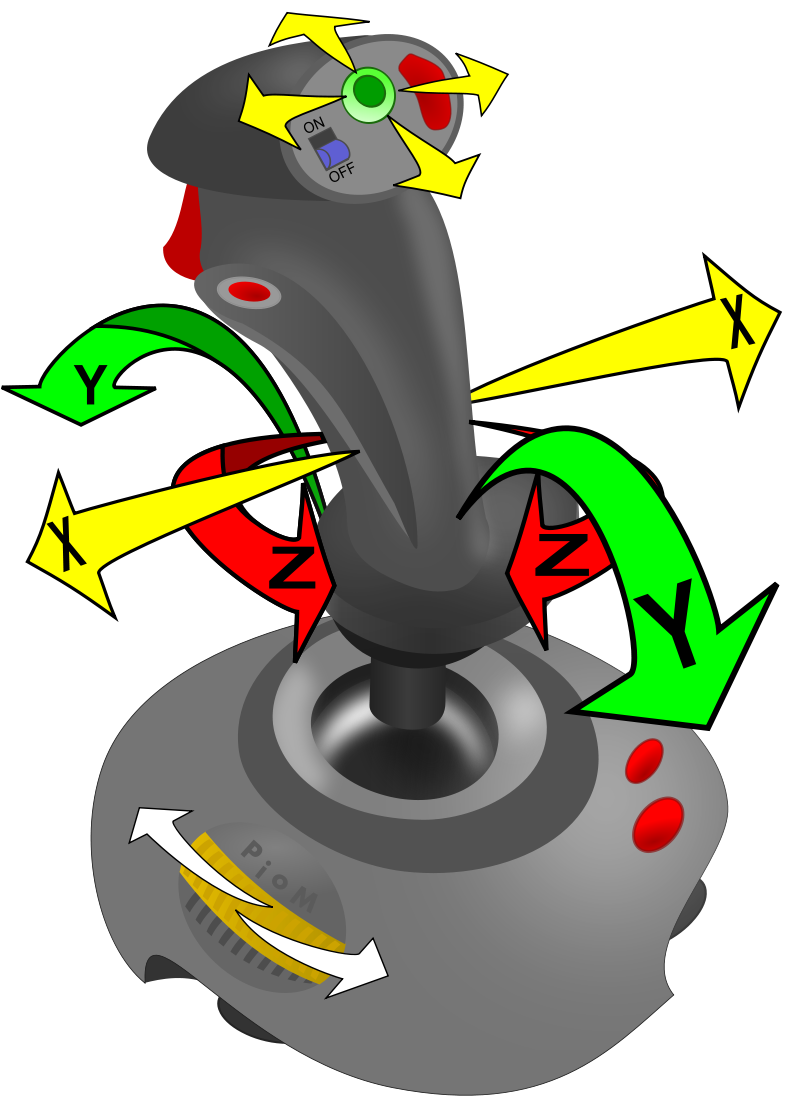
\includegraphics[width=0.3\textwidth]{"media/Wikipedia_Joystick.png"}
			\caption{Joystick from Wikipedia \cite{web:wiki:Joystick}}
			\label{fig:Wikipedia Joystick}
		\end{wrapfigure}
		A Joystick which only has rotational axes. These are commercially available and find wide spread use in industrial as well as entertainment industries.
	}
	
	\chapter{Hardware}
	\section{Goals}
		Allow for translation and rotation of a joystick such that each axis can be controlled without influencing the other axes.
		All Axes should be controlled using one hand, without taking the hand of the stick.
		
	\section{Preliminary Design Exploration}
		\subsection{Stick with Gyroscopes}
			A stick with several Gyroscopes attached.
			Each Gyroscope is tracking its position and rotation in space.
			On first implementation major precision issues were encountered resulting in drift for slow movements, which are necessary for precise control of vehicles.
		\subsection{Joystick on Rails}
			\begin{wrapfigure}{r}{0.45\textwidth}
				\includegraphics[width=0.45\textwidth]{"media/Joystick_on_Rails_v5"}
				\caption{The Joystick on Rails design with one side of the necessary rails and connecting pieces, the joystick which does rotations is missing in the depiction}
				\label{fig:v5}
			\end{wrapfigure}
			Putting a normal Joystick on rails like a 3D-Print head seemed like a good approach to get a working prototype. 5 Linear Axes would be arranged like in a standard 3D Printer. 2 Supporting Z Axis (up and down movement) on the left and right side of the \refdefinition{Actuation Space}  (only the left pictured in \reffigure{v5}), then two more to support the Y Axis (front to back movements), and the last to support x (left right movements). At the center there would be a standard commercially available \refdefinition{3DOF Joystick} for rotational inputs.
	
	\newpage
	\listoffigures
	\newpage
	\listoftables
	\newpage
	\bibliographystyle{abbrv}
	\bibliography{design_doc}
\end{document}